% main.tex — theoretical companion to denote (Overleaf-ready: upload this folder; compiler pdfLaTeX)
\documentclass[11pt,a4paper]{article}
\usepackage[utf8]{inputenc}
\IfFileExists{lmodern.sty}{\usepackage[T1]{fontenc}\usepackage{lmodern}}{\PassOptionsToPackage{expansion=false}{microtype}}% Latin Modern where available (e.g. Overleaf)
\usepackage[margin=2.4cm]{geometry}
\usepackage{amsmath,amssymb,amsthm}
\usepackage{stmaryrd}
\usepackage[round,authoryear]{natbib}
\usepackage{booktabs,tabularx,array}
\usepackage[shortlabels]{enumitem}
\usepackage{microtype}
\usepackage{xcolor}
\usepackage{tikz}
\usetikzlibrary{arrows.meta}
\usepackage[colorlinks=true,linkcolor=blue!45!black,citecolor=green!35!black,urlcolor=blue!60!black]{hyperref}

\setlist{itemsep=1pt,topsep=3pt}
\newcommand{\den}[1]{\llbracket #1\rrbracket}
\newcommand{\dn}{\textsf{denote}}
\newcommand{\ty}[1]{\langle #1\rangle}
\newcommand{\cmd}[1]{\texttt{#1}}
\newcolumntype{L}{>{\raggedright\arraybackslash}X}
\newtheorem{definition}{Definition}
\newtheorem{proposition}{Proposition}
\theoremstyle{definition}
\newtheorem{vignette}{Vignette}

\title{The Theory Behind \dn{}:\\[2pt] \large Foundations, Lenses, and Related Work for an Executable Compositional Semantics}
\author{The \dn{} contributors}
\date{Companion document to \dn{} v0.1.0 \quad$\cdot$\quad October 2026}

\begin{document}
\maketitle

\begin{abstract}
\noindent\dn{} is a type-driven workbench for compositional model-theoretic semantics. Given a lexicon of typed $\lambda$-terms and a constituency tree, it computes the set of $\beta$-normal denotations licensed by the composition principles of the Heim--Kratzer tradition, records every contraction, and submits the results to model checking, presupposition projection, alternative-semantic analysis, tests of generalized-quantifier universals, polarity profiling, bounded inference and a family of model-theoretic statistics. This document is the theoretical companion to the software. It reconstructs the lineage of each module, from the Fregean and Church--Montague foundations, through type-driven interpretation, type flexibility and four rival theories of quantifier scope, to trivalent theories of projection, alternative semantics, generalized-quantifier theory, polarity, logical probability and computational inference. It also makes explicit which commitments the software hard-codes, which it exposes as interchangeable \emph{lenses}, and which it leaves out. Where the software's outputs bear on live debates (the expressive limits of one-level continuations, spurious scope ambiguity, the proviso problem, quantified presuppositions, Strawson entailment and NPI licensing), the results are reported as short, reproducible vignettes.
\end{abstract}

\tableofcontents
\bigskip

% ═══════════════════════════════════════════════════════════════════════════════
\section{Introduction}\label{sec:intro}

Since \citet{montague1970efl,montague1970ug,montague1973}, natural-language semantics has been practised as a discipline of explicit construction. A fragment is specified by a syntactic algebra, a lexicon and a homomorphic mapping into a model-theoretic algebra, and every claim about meaning is a claim about what that construction delivers \citep{dowtywallpeters1981,gamut1991,parteehendriks1997,partee2011}. The type-driven reformulation of the programme \citep{kleinsag1985,heimkratzer1998} made the construction \emph{locally} computable: the semantic types of a node's daughters determine which combinatory principle applies. \dn{} takes that computability literally. It executes the interpretation function on a given tree and keeps the full reduction trace. It then treats the resulting denotations as objects of further mathematical study: it evaluates them in finite models, computes their projected presuppositions, compares them under entailment, and measures how often rival readings come apart.

This document has two aims. The first is genealogical: to situate each component of the software in the literature from which it derives, in enough detail that a reader can reconstruct the theoretical commitments the code inherits. The second is critical: to state where the software adjudicates between rival analyses, where it merely exposes them side by side, and where it is silent. We organise the second aim around the notion of a \emph{lens}.

\paragraph{Lenses.} A lens is a parameterised family of interpretive commitments that can be exchanged while the remainder of a grammar (lexicon, trees, models) is held fixed (Table~\ref{tab:lenses}). The methodological point is familiar from the debate on compositionality \citep{partee1984,janssen1997}. Analyses of the syntax--semantics interface are underdetermined by any single derivation, and are distinguished only by the \emph{sets} of derivations they license across a body of data. Executable lenses turn such comparisons from rhetorical exercises into mechanical ones. The same tree is interpreted under each commitment, and the outputs are compared both derivationally (which readings, by which rules) and model-theoretically (in which models they diverge).

\begin{table}[t]\centering\small
\caption{Lenses exposed by \dn{}: interchangeable commitments evaluated against a fixed grammar.}\label{tab:lenses}
\begin{tabularx}{\textwidth}{@{}lLL@{}}
\toprule
Dimension & Options & Principal sources\\
\midrule
Scope-taking & Quantifier Raising; Cooper storage; one-level continuations; argument raising & \citet{may1977,may1985}; \citet{cooper1983}; \citet{barker2002}; \citet{hendriks1993}\\
Type economy & no shifting; last resort; free shifting & \citet{parteerooth1983}; \citet{partee1987}; \citet{chierchia1998}\\
Definite article & Frege--Strawson $\iota$ (partial); Russellian quantifier (total) & \citet{frege1892}; \citet{strawson1950}; \citet{russell1905}; \citet{heim1991}\\
Projection & weak (Bochvar), strong (Kleene) and middle (Peters) trivalent schemes & \citet{bochvar1938}; \citet{kleene1952}; \citet{peters1979}; \citet{george2008}\\
Entailment & classical; Strawson & \citet{vonfintel1999}\\
Focus & structured meanings; Roothian alternative sets & \citet{vonstechow1990}; \citet{krifka1991}; \citet{rooth1985,rooth1992}\\
\bottomrule
\end{tabularx}
\end{table}

\begin{table}[t]\centering\small
\caption{Modules of \dn{}, the formal objects they implement, and their principal antecedents.}\label{tab:modules}
\begin{tabularx}{\textwidth}{@{}lLLc@{}}
\toprule
Module & Formal object & Antecedents & \S\\
\midrule
\cmd{typesys}, \cmd{typecheck} & simple types over $e,t,s,v,i,d$; unification & \citet{church1940,gallin1975,hindley1969,milner1978} & \ref{sec:substrate}\\
\cmd{terms}, \cmd{reduce} & the term language $\Lambda$; $\beta\eta\partial$-reduction & \citet{church1936,churchrosser1936,tait1967,debruijn1972} & \ref{sec:substrate}\\
\cmd{compose} & type-driven rules; type-shifters; lenses & \citet{kleinsag1985,heimkratzer1998,partee1987,hendriks1993} & \ref{sec:typedriven}--\ref{sec:flex}\\
\cmd{scope} & LF generation; reading pools & \citet{may1977,cooper1983,barker2002} & \ref{sec:scope}\\
\cmd{models}, \cmd{projection} & trivalent model theory; bilateral translation & \citet{kleene1952,peters1979,karttunen1974,kripke1975} & \ref{sec:presup}\\
\cmd{analysis.gq} & GQ universals; positional polarity & \citet{barwisecooper1981,keenanstavi1986,vanbenthem1986,ladusaw1979} & \ref{sec:gq}--\ref{sec:polarity}\\
\cmd{analysis.ambiguity}, \cmd{metrics} & measures on finite model classes & \citet{carnap1950,carnapbarhillel1952,fagin1976} & \ref{sec:measure}\\
\cmd{analysis.inference}, \cmd{export} & bounded entailment; prover export & \citet{cooperetal1996,blackburnbos2005,sutcliffe2009} & \ref{sec:inference}\\
\bottomrule
\end{tabularx}
\end{table}

\begin{figure}[t]\centering
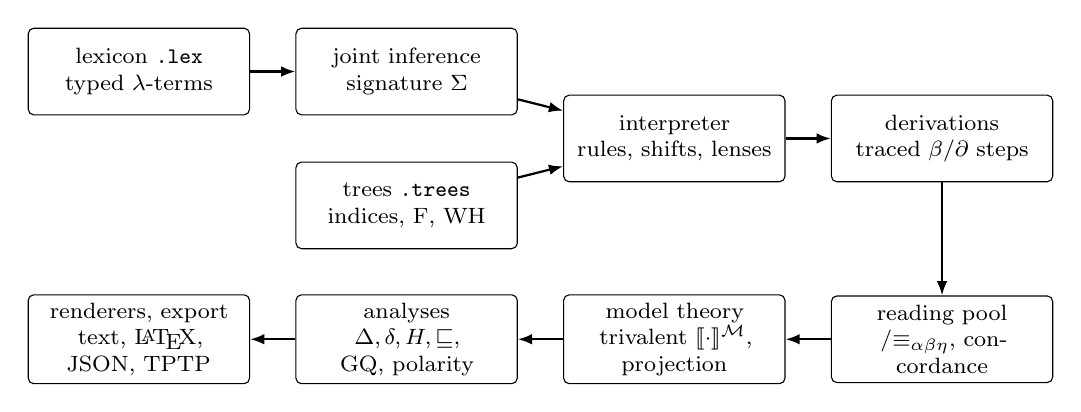
\begin{tikzpicture}[box/.style={draw,rounded corners=2pt,align=center,font=\footnotesize,inner sep=3pt,text width=26mm,minimum height=11mm},arr/.style={-{Latex[length=1.8mm]},thick}]
\node[box] (lex) at (0,0) {lexicon \cmd{.lex}\\typed $\lambda$-terms};
\node[box] (sig) at (3.4,0) {joint inference\\signature $\Sigma$};
\node[box] (tree) at (3.4,-1.7) {trees \cmd{.trees}\\indices, F, WH};
\node[box] (int) at (6.8,-0.85) {interpreter\\rules, shifts, lenses};
\node[box] (der) at (10.2,-0.85) {derivations\\traced $\beta/\partial$ steps};
\node[box] (pool) at (10.2,-3.4) {reading pool\\$/{\equiv_{\alpha\beta\eta}}$, concordance};
\node[box] (mod) at (6.8,-3.4) {model theory\\trivalent $\den{\cdot}^{\mathcal M}$, projection};
\node[box] (ana) at (3.4,-3.4) {analyses\\$\Delta,\delta,H,\sqsubseteq$, GQ, polarity};
\node[box] (out) at (0,-3.4) {renderers, export\\text, \LaTeX, JSON, TPTP};
\draw[arr] (lex)--(sig); \draw[arr] (sig)--(int); \draw[arr] (tree)--(int); \draw[arr] (int)--(der);
\draw[arr] (der)--(pool); \draw[arr] (pool)--(mod); \draw[arr] (mod)--(ana); \draw[arr] (ana)--(out);
\end{tikzpicture}
\caption{Architecture of \dn{}. The upper row constructs meanings; the lower row analyses them.}\label{fig:arch}
\end{figure}

\paragraph{Contributions.} The software makes four contributions.
\begin{enumerate}[(i)]
\item A \emph{mechanism concordance}. Readings derived by QR, storage, continuations and argument raising are pooled modulo $\alpha\beta\eta$-equivalence and annotated with the mechanisms that derive them, so that differences in generative capacity become observable data (\S\ref{sec:scope}).
\item A small family of \emph{model-theoretic statistics}, computed over finite model classes: scope sensitivity, a disagreement pseudometric, profile entropy, an entailment preorder and Bar-Hillel--Carnap informativity (\S\ref{sec:measure}).
\item Symbolic \emph{presupposition projection} under three trivalent schemes, via a bilateral translation whose adequacy is stated as a proposition and checked by property-based testing (\S\ref{sec:presup}).
\item \emph{Executable theory comparison}: competing lexicons are scored against a shared suite of entailment, ambiguity and truth-value items (\S\ref{sec:engineering}).
\end{enumerate}
None of the underlying theories is new. What is new is their co-presence in a single, inspectable artefact whose outputs can be compared along every lens at once.

% ═══════════════════════════════════════════════════════════════════════════════
\section{Compositionality and the architecture of interpretation}\label{sec:comp}

\subsection{The principle and its formal reconstructions}
The principle that the meaning of a complex expression is determined by the meanings of its parts and their mode of combination bears Frege's name. The attribution is contested, and the principle admits many non-equivalent formulations \citep{janssen1997,paginwesterstahl2010}. \citet{montague1970ug} gives it algebraic form. Syntax is a many-sorted algebra $\mathfrak{A}=\ty{A,F_\gamma}_{\gamma\in\Gamma}$, meanings form an algebra $\mathfrak{B}$ of the same signature, and interpretation is a homomorphism $h:\mathfrak{A}\to\mathfrak{B}$, so that $h(F_\gamma(a_1,\dots,a_n))=G_\gamma(h(a_1),\dots,h(a_n))$. \citet{janssen1997} develops this conception in detail, and \citet{hodges2001} gives a general framework in which compositionality, its variants and their interrelations can be stated and proved.

The principle's empirical bite has been questioned. \citet{zadrozny1994} showed that any assignment of meanings can be recast compositionally by a suitable encoding. \citet{westerstahl1998} replied that such results trivialise the principle only if the syntactic algebra and the meanings may be chosen freely, and that the constraint has content once both are fixed independently. \citet{partee1984} treats compositionality as a methodological working hypothesis whose value lies in the discipline it imposes on analyses. \dn{} adopts Westerst{\aa}hl's position in operational form: the tree (a term of the syntactic algebra) and the lexicon are fixed inputs, and the rule inventory is a small, closed set. Interpretation is then a structural recursion
\begin{equation}\label{eq:interp}
\den{\cdot}:\mathrm{Tree}\to\wp_{\mathrm{fin}}(\Lambda),\qquad
\den{[_X\,\beta\ \gamma]}=\bigcup_{R\in\mathcal{R}}\big\{R(b,c)\;\big|\;b\in\den{\beta},\ c\in\den{\gamma},\ R(b,c)\!\downarrow\big\}\big/{\equiv_\alpha},
\end{equation}
where $\mathcal{R}$ is the active rule set and $R(b,c)\!\downarrow$ means that $R$ is defined on the types of $b$ and $c$. Set-valuedness is the standard device for reconciling ambiguity with compositionality \citep{janssen1997}. Ambiguity can then be located in the lexicon (sense-tagged homonyms), in the tree (distinct logical forms), or in the choice of rule (the lenses of Table~\ref{tab:lenses}).

\subsection{Direct and indirect interpretation}
\citet{montague1970efl} interprets English directly in a model. \citet{montague1973} instead translates it into intensional logic and interprets the translation, noting that the intermediate language is dispensable in principle; \citet{lewis1970} defends a direct, categorial variant. Contemporary \emph{direct compositionality} \citep{barkerjacobson2007,jacobson2014} pairs each syntactic rule with a semantic operation and dispenses with a level of logical form. The LF tradition \citep{may1977,may1985,heimkratzer1998} instead interprets a syntactically transformed representation. \dn{} is indirect in Montague's sense and LF-based in May's: trees are inputs, and the \cmd{scope} module manufactures logical forms.

The intermediate language is retained for two reasons. Pedagogically, it is the medium in which textbook derivations are written \citep{dowtywallpeters1981,gamut1991,heimkratzer1998}. Computationally, equivalence of simply typed terms modulo $\alpha\beta\eta$ is decidable by normalisation, whereas model-theoretic equivalence of first-order formulas is not \citep{church1936note}. $\equiv_{\alpha\beta\eta}$ therefore serves as a sound but incomplete proxy for synonymy, supplemented by bounded model-theoretic checks (\S\ref{sec:measure}).

% ═══════════════════════════════════════════════════════════════════════════════
\section{The logical substrate}\label{sec:substrate}

\subsection{Simple types and their sorts}
\dn{}'s type system is Church's simple theory of types \citep{church1940} over six basic sorts:
\begin{equation}
\mathcal{T}::= e\mid t\mid s\mid v\mid i\mid d\mid\ty{\mathcal{T},\mathcal{T}}\mid {}'a,\qquad D_{\ty{\sigma,\tau}}=D_\tau^{\,D_\sigma}.
\end{equation}
Worlds appear as an explicit sort, as in Gallin's two-sorted $\mathrm{Ty}_2$, rather than through the $^\wedge/^\vee$ operators of Montague's intensional logic \citep{gallin1975}; on the relationship between the two systems see \citet{gallin1975} and \citet{zimmermann1989}. Eventualities ($v$) follow \citet{davidson1967} and \citet{parsons1990}; degrees ($d$) follow \citet{cresswell1976}; times ($i$) follow the index-based tradition of \citet{montague1973}. Type variables $'a$ are rigid within a lexical entry and renamed apart across entries. They provide the schematic polymorphism of cross-categorial operators such as generalized conjunction \citep{parteerooth1983} and focus-sensitive particles \citep{rooth1985}, not the let-polymorphism of ML \citep{milner1978}.

Models are \emph{standard} over finite domains. $D_{\ty{\sigma,\tau}}$ is the full function space, so quantification over $\ty{\sigma,t}$ ranges over the entire power set of $D_\sigma$, not over a Henkin-style general model \citep{henkin1950}. Non-logical constants, however, are interpreted only at first-order types, and higher-order lexical meanings must be defined by $\lambda$-terms over first-order relations. This keeps model enumeration finite and makes export to first-order provers possible (\S\ref{sec:inference}).

\subsection{The term language and its metatheory}
The term language $\Lambda$ is the simply typed $\lambda$-calculus \citep{church1936,church1940} enriched with logical constants, the variable-binding operators $\forall$, $\exists$ and $\iota$, a maximality operator \textsc{max}, a cardinality operator, and a definedness operator $\partial$. Traces are produced by normal-order reduction, and three classical results justify this choice:
\begin{itemize}
\item by the Church--Rosser theorem \citep{churchrosser1936}, normal forms are unique;
\item by strong normalisation of the simply typed calculus \citep{tait1967}, every reduction sequence terminates;
\item by the standardisation theorem \citep{barendregt1984}, leftmost-outermost reduction reaches the normal form whenever one exists, which yields the canonical textbook derivation \citep{hindleyseldin2008}.
\end{itemize}
Substitution is capture-avoiding, with renaming by priming. $\alpha$-equivalence is decided on nameless keys in the manner of \citet{debruijn1972}.

\subsection{Partiality}
On the view of \citet{frege1892} and \citet{strawson1950}, an expression whose presupposition fails lacks a truth value rather than being false. \citet{heimkratzer1998} encode this with partial functions, written $\lambda x:\varphi.\,M$ and defined only for arguments that satisfy $\varphi$. \dn{} internalises the domain condition as a term former $\partial[\varphi]M$, which denotes $\den{M}$ if $\den{\varphi}=1$ and is undefined otherwise. At type $t$ this is Blamey's \emph{transplication} \citep{blamey1986}; with a trivial second argument it is the unary presupposition operator $\partial\varphi$ of \citet{beaverkrahmer2001}. Two strictness rules propagate it through application: $(\partial[\varphi]F)N\rightsquigarrow\partial[\varphi](FN)$, and $F(\partial[\varphi]N)\rightsquigarrow\partial[\varphi](FN)$ for $F$ not an abstraction. As a result, presuppositions surface at the clause level in normal forms. \citet{muskens1995} develops a fully partial type theory, with four truth values and partial functions at every type. \dn{} restricts partiality to three sources ($\iota$, \textsc{max} and $\partial$) and evaluates with a single third value, $\#$.

\subsection{Type inference}
Types are reconstructed by first-order unification \citep{robinson1965}, in the manner of principal type-schemes \citep{hindley1969} and Algorithm~W \citep{milner1978} but without generalisation. Residual type variables are resolved in three steps:
\begin{enumerate}[1.]
\item by the notational conventions of the literature: $x,y,z{:}e$; $P,Q{:}\ty{e,t}$; $R{:}\ty{e,\ty{e,t}}$; $p,q{:}\ty{s,t}$; $w{:}s$; $e{:}v$; $d{:}d$;
\item by giving non-logical constants the result type $t$;
\item by assigning $e$ to anything that remains.
\end{enumerate}
All entries of a lexicon are typed \emph{jointly}, so every non-logical constant receives a single type and the lexicon determines a signature $\Sigma:\mathrm{Const}\to\mathcal{T}$. The defaulting is a heuristic that encodes textbook conventions \citep{heimkratzer1998,coppockchampollion2024}; explicit annotations always take precedence.

% ═══════════════════════════════════════════════════════════════════════════════
\section{Type-driven interpretation and the syntax--semantics interface}\label{sec:typedriven}

\subsection{From rule-to-rule to type-driven translation}
Montague's grammars pair each syntactic rule with a dedicated translation rule. \citet{kleinsag1985} replaced this pairing with a small set of \emph{type-driven} principles that apply whenever the types of the daughters permit, and \citet{bittner1994} used the same architecture to state cross-linguistic generalisations. \citet{heimkratzer1998} fixed the now-canonical inventory: Terminal Nodes, Non-branching Nodes, Functional Application, Predicate Modification and Predicate Abstraction. Alongside it they state the \emph{Principle of Interpretability}, which requires every node of a tree to be in the domain of the interpretation function. Textbook presentations of the same architecture include \citet{chierchiamcg2000}, \citet{winter2016} and \citet{coppockchampollion2024}. \citet{jacobson2014} presents the alternative, direct-compositional system and compares the two at length.

\subsection{Predicate Modification and its descendants}
Predicate Modification, the conjunction of two predicates of the same argument, is the type-driven heir of the $\theta$-identification of \citet{higginbotham1985}. \citet{kratzer1996} generalised the idea to Event Identification, by which a Voice head of type $\ty{e,\ty{v,t}}$ conjoins with an event predicate. \dn{} implements both, with PM generalised to any type $\ty{\sigma,t}$.

\subsection{Intensional Functional Application}
Suppose a functor $\beta:\ty{\ty{s,\sigma},\tau}$ expects an intension, and its sister $\gamma:\sigma$ denotes an extension. Intensional Functional Application then abstracts over the evaluation world: $\den{\alpha}=\den{\beta}(\lambda w.\den{\gamma})$. The rule, and the use of object-language world variables, follow \citet[ch.~12]{heimkratzer1998} and \citet{vonfintelheim2011}. Root clauses of type $\ty{s,t}$ are saturated by the free evaluation-world variable $w$.

\subsection{Movement, indices and assignments}
Traces and pronouns denote assignment-dependent individuals, and a numerical binder index above a constituent triggers Predicate Abstraction over the corresponding variable \citep[chs.~5, 7, 9]{heimkratzer1998}. In \dn{} the assignment function is represented syntactically: an indexed leaf $t_i$ translates to a variable $x_i$, and PA is $\lambda$-abstraction over $x_i$. Free variables that survive to the root are evaluated against the model's assignment $g$. The well-formedness constraint of \citet{partee1979wfc}, which bars level-skipping transformations of this kind, has no direct counterpart: \dn{} interprets whatever trees it is given, and leaves the choice between LF-based and surface-based architectures to the user.

\subsection{Coordination}
Generalized conjunction \citep{parteerooth1983} defines $\sqcap$ pointwise on all types that end in $t$, and \citet{winter2001} develops the Boolean architecture behind it. \dn{} implements pointwise meet and join. It also implements Partee and Rooth's strategy of raising a conjunct of type $e$ to the generalized-quantifier type when the other conjunct requires it, so that \textit{Rex and every cat} composes as $\lambda P.P(\textit{rex})\wedge\forall x[\textit{cat}(x)\to P(x)]$.

\subsection{Interpretability failure as data}
A composition failure is itself informative. The paradigm case is a quantifier in object position, which is uninterpretable in situ because neither $\ty{e,\ty{e,t}}$ nor $\ty{\ty{e,t},t}$ can apply to the other. \citet[ch.~7]{heimkratzer1998} present two repairs, QR and type-shifting the verb, and the subsequent literature adds storage and continuations. \dn{} turns this dialectic into a diagnostic. It reports the offending node and the clashing types, and it lists the repairs under which the node would become interpretable.

\begin{vignette}[object quantifiers]\label{v:object}
With type-shifting disabled, \textit{Rex chased every cat} fails at VP with the clash $\ty{e,\ty{e,t}}$ versus $\ty{\ty{e,t},t}$. The diagnosis proposes QR, Cooper storage, continuations and argument raising. Under the default economy setting the object composes by argument raising \citep{hendriks1993}, yielding $\forall x'[\textit{cat}(x')\to\textit{chase}(\textit{rex},x')]$.
\end{vignette}

% ═══════════════════════════════════════════════════════════════════════════════
\section{Type flexibility and its economy}\label{sec:flex}

\subsection{The type-shifting triangle}
\citet{partee1987} organised the interpretation of noun phrases around the types $e$, $\ty{e,t}$ and $\ty{\ty{e,t},t}$ and the natural maps between them. These include \textsf{LIFT} ($a\mapsto\lambda P.P(a)$), \textsf{IDENT} ($a\mapsto\lambda x.x=a$), \textsf{iota}, \textsf{A} (existential closure of a property) and \textsf{BE} ($\mathcal{Q}\mapsto\lambda x.\mathcal{Q}(\lambda y.y=x)$). Partee argued that \textsf{BE} is privileged because it is a homomorphism from generalized quantifiers to properties. \citet{chierchia1998} added kind-forming shifts and the \emph{blocking principle}, by which a covert shift is unavailable where an overt determiner performs the same function. \dn{} implements \textsf{LIFT}, \textsf{IDENT}, \textsf{IOTA}, \textsf{A} and \textsf{BE}.

\begin{vignette}[the copula]\label{v:copula}
If the copula is an identity function on properties, \textit{Rex is a dog} is interpretable only if the generalized quantifier \textit{a dog} is mapped to a property. \dn{} applies \textsf{BE} as a last resort and derives $\exists x[\textit{dog}(x)\wedge x=\textit{rex}]$, which is Partee's analysis of predicative indefinites.
\end{vignette}

\subsection{Flexible types}
\citet{hendriks1993} generalised type-shifting to three rules, value raising, argument raising and argument lowering. He showed that scope ambiguity can be derived in situ, with each order of argument raising corresponding to a scoping. \dn{} implements argument raising for transitive relations in two scopal variants, object-narrow and object-wide.

\subsection{Categorial and variable-free alternatives}
The categorial tradition derives type-shifting from a logic of syntactic types. \citet{lambek1958} gave the calculus, and \citet{vanbenthem1991} systematised the correspondence between categorial derivations and $\lambda$-terms, including results on how many readings a sequent admits. Combinatory Categorial Grammar \citep{steedman2000} restricts the available combinators (composition, type-raising and substitution) and makes them sensitive to linear order. The composition rule of \citet{geach1972} is the cornerstone of the variable-free semantics of \citet{jacobson1999}, in which binding is effected by combinators rather than by assignments.

\subsection{Economy}
How much shifting a grammar may do is a substantive hypothesis. \citet{parteerooth1983} proposed that expressions are entered at their lowest type and raised only when composition demands it, and \citet{partee1987} formulated shifting as a last resort. On independent grounds, \citet{fox2000} argued that scope-shifting operations are licensed only if they have a semantic effect. \dn{} exposes three economy settings: \texttt{off}, \texttt{last-resort} and \texttt{free}. The statistics of \S\ref{sec:measure} connect directly with Fox's condition. Readings in a single model-theoretic equivalence class are precisely those between which a scope shift would have no effect, at least on the finite models examined.

\begin{vignette}[the cost of non-directional composition]\label{v:fc}
Suppose Geach composition is freely available in a type-driven system without directional syntax. A transitive verb can then compose with an object quantifier in a way that reverses the verb's thematic roles, so that \textit{every student read a book} receives a reading on which books read students. Directional categorial systems \citep{lambek1958,steedman2000,jacobson1999} block this by word order. \dn{} therefore makes function composition opt-in (\texttt{--allow FC}).
\end{vignette}

% ═══════════════════════════════════════════════════════════════════════════════
\section{Quantifier scope: four lenses and their concordance}\label{sec:scope}

\subsection{Quantifying-in and Quantifier Raising}
\citet{montague1973} derived scope ambiguity by \emph{quantifying in}: a sentence containing a variable is combined with a noun phrase that binds it, in any order. \citet{may1977,may1985} recast the idea as a movement operation at Logical Form. Quantifier Raising adjoins a quantificational DP to a clausal node and leaves a coindexed trace. \citet[chs.~7--8]{heimkratzer1998} give its type-driven semantics, with the movement index interpreted by Predicate Abstraction. For each permutation of the quantificational DPs, \dn{} generates an LF in which each DP is adjoined to its nearest clause, or to the root under \texttt{--unbounded}. Derivations in which a QR trace escapes its binder, as when a container raises above its own contents, are filtered out.

\subsection{Storage}
\citet{cooper1983} achieved scope ambiguity without movement. A quantifier may be replaced in situ by a variable and placed in a store, from which it is retrieved at any node of type $t$ by applying it to the abstraction over its variable. In nested configurations, retrieval in the wrong order leaves a variable unbound, and \citet{keller1988} introduced \emph{nested} storage to exclude such derivations. \dn{} implements unnested storage and counts the ill-formed retrieval orders, which therefore become an observable signature of Keller's problem.

\subsection{Continuations}
\citet{barker2002} showed that quantifiers can be treated as functions on their own continuations, with scope ambiguity arising from the order in which the computations of sister constituents are evaluated. \citet{shanbarker2006} derived crossover and superiority effects from a default left-to-right evaluation order. \citet{barkershan2014} developed the multi-level \emph{tower} system, and \citet{charlow2020} uses a monadic generalisation to account for the exceptional scope of indefinites. \dn{} implements a deliberately one-level system:
\begin{itemize}
\item a daughter of type $\ty{\ty{\sigma,t},t}$ may be read as a computation of a $\sigma$;
\item values combine by Functional Application or Predicate Modification inside the continuation monad;
\item either daughter may be evaluated first;
\item computations of type $t$ are lowered.
\end{itemize}

\subsection{Flexible types, choice functions and exceptional scope}
Argument raising \citep{hendriks1993} provides the fourth mechanism (\S\ref{sec:flex}). A fifth family, which \dn{} does not implement, treats indefinites by choice functions \citep{reinhart1997,winter1997}. It is motivated by the island-violating, apparently referential readings identified by \citet{fodorsag1982}. \citet{charlow2020} offers an alternative-based reconstruction of the same data.

\subsection{Enumeration, underspecification and redundancy}
Computational semantics confronted the combinatorics of scope early. \citet{hobbsshieber1987} gave an algorithm that enumerates well-formed scopings directly, while underspecified representations such as UDRT \citep{reyle1993} and Minimal Recursion Semantics \citep{copestakeetal2005} postpone enumeration altogether. Because many scopings are truth-conditionally redundant, \citet{vestre1991} designed an enumeration that avoids equivalent permutations. \citet{kollerthater2010} compute the \emph{weakest} readings of an underspecified description by eliminating readings that entail others. \dn{}'s model-theoretic equivalence classes and entailment Hasse diagram are a semantic, bounded analogue of these syntactic techniques: equivalence and entailment are tested in finite models rather than established by rewriting.

\subsection{Ambiguity, entailment and the weakest-reading hypothesis}
When one reading entails another, the standard tests for ambiguity behave unreliably \citep{zwickysadock1975}. \citet{kempsoncormack1981} asked whether such scope ``ambiguities'' are genuine, or reduce to a single weak reading. The entailment preorder computed by \dn{} makes the relevant structure explicit for any sentence. It identifies the weakest and the strongest readings, and the disagreement metric measures how far apart they lie.

\subsection{Empirical preferences}
Experimental and corpus work treats scope as a graded preference. \citet{kurtzmanmacdonald1993} measured scope resolution in comprehension, and \citet{higginssadock2003} trained classifiers on corpus-annotated scope preferences. \citet{szabolcsi2010} surveys the range of scope-taking strategies across quantifier types. \dn{} derives the possible readings, not their preferences, so its outputs can serve as the hypothesis space for such models.

\begin{vignette}[concordance and spurious ambiguity]\label{v:spurious}
For \textit{every student read a book}, all four mechanisms derive both readings, and the inverse reading entails the surface one ($\rho_2\models\rho_1$). For \textit{every student read every book}, they again derive two terms that differ modulo $\equiv_{\alpha\beta\eta}$. These terms, however, fall into a single model-theoretic equivalence class ($\Delta=0$). This is the paradigm of spurious ambiguity: redundancy-eliminating algorithms remove it \citep{vestre1991}, and Scope Economy excludes it \citep{fox2000}.
\end{vignette}

\begin{vignette}[the limits of one continuation level]\label{v:cont}
For \textit{every student showed a professor two books}, QR and storage derive all $3!=6$ readings, while the one-level continuation lens derives four. The two missing readings are those in which the subject takes scope between the two objects. At the VP node, the computations of the two objects are sequenced into a single computation of a property, whose internal order is fixed before the subject is evaluated. The subject can therefore scope above or below this block, but not inside it. This is the expected limitation of a single continuation level, which multi-level towers \citep{barkershan2014} are designed to overcome.
\end{vignette}

\begin{vignette}[inverse linking]\label{v:inverse}
For \textit{a student from every country left}, clause-bounded QR, storage and continuations derive only the inverse-linked reading ($\forall$ over $\exists$). One storage retrieval order is discarded as ill-formed, which is the configuration that motivated nested storage \citep{keller1988}. Only argument raising yields the surface reading. Admitting DP-internal landing sites for QR, as suggested by the evidence that DP is not a scope island \citep{may1985,sauerland2005}, would let QR derive both.
\end{vignette}

% ═══════════════════════════════════════════════════════════════════════════════
\section{Intensionality, modality and attitudes}\label{sec:intensional}

Three ideas entered linguistics with \citet{montague1973}: the method of intension and extension \citep{carnap1947}, possible-worlds semantics for modality \citep{kripke1963}, and possible-worlds semantics for attitudes \citep{hintikka1969}. Gallin's $\mathrm{Ty}_2$ made world-dependence explicit in the object language \citep{gallin1975}, and \citet{vonfintelheim2011} systematised the use of world variables and Intensional Functional Application within the Heim--Kratzer framework. \dn{}'s intensional fragment treats modals as quantifiers over worlds accessible from the evaluation world. This is the degenerate case of Kratzer's theory, with a modal base and no ordering source \citep{kratzer1977,kratzer2012}. Attitude verbs are treated as universal quantifiers over doxastic alternatives \citep{hintikka1969}.

\paragraph{De re and de dicto.} \citet{quine1956} distinguished the relational from the notional reading of \textit{Ralph believes that someone is a spy}, and \citet{fodor1970} showed that the specific/non-specific and transparent/opaque distinctions cross-classify. On the scope theory, de re readings arise when the DP takes scope over the attitude verb. \citet{percus2000} argued that scope alone both under- and over-generates, and that the world arguments of predicates must be represented and bound under structural constraints of their own. \dn{}'s world-variable architecture is compatible with Percus's alternative, although the shipped lexicon implements the scope theory.

\begin{vignette}[de re]\label{v:dere}
For \textit{John believes that a spy left}, clause-bounded QR and one-level continuations derive only the de dicto reading, since neither can move the indefinite out of the complement clause. Cooper storage, which retrieves at any node of type $t$, and unbounded QR also derive the de re reading $\exists x[\textit{spy}(w,x)\wedge\forall v[\textit{dox}(\textit{john},w,v)\to\textit{leave}(v,x)]]$. The concordance thus makes explicit a fact that usually remains implicit: which mechanisms are clause-bounded.
\end{vignette}

\paragraph{Intensional transitive verbs.} \citet{montague1973} analysed \textit{seek} as \textit{try to find}, which gives the object a notional reading under the intensional operator. \citet{zimmermann1993} argued that opaque verbs take properties rather than intensional quantifiers as objects. The shipped entry follows Montague. Because \dn{} types lexicons jointly and compares outputs mechanically, Zimmermann's property-based entry can be substituted and the two analyses compared on the same trees.

\paragraph{Factives and hyperintensionality.} Factive verbs presuppose their complements \citep{kiparsky1970}. \dn{} encodes \textit{know} with a domain condition, and its presupposition projects through negation under all three schemes (\S\ref{sec:presup}). The model theory is intensional but not hyperintensional: logically equivalent complements are intersubstitutable under \textit{believe}. This is the familiar objection to possible-worlds treatments of attitudes, and it is the problem that structured meanings address \citep{cresswell1985}.

% ═══════════════════════════════════════════════════════════════════════════════
\section{Events}\label{sec:events}

\citet{davidson1967} argued that action sentences quantify over events. Adverbial modifiers then become conjoined predicates of an event, and the entailments among modified sentences follow from conjunction elimination. \citet{parsons1990} added thematic-role predicates, giving the neo-Davidsonian format. \citet{kratzer1996} severed the external argument from the verb and introduced it by a Voice head that combines by Event Identification. \citet{landman2000} develops the theory of events and plurality. \citet{champollion2015} identifies a systematic problem in the interaction of event semantics with quantifiers and negation, and resolves it by letting verbs denote existential quantifiers over events.

\begin{vignette}[Davidson's diamond]\label{v:diamond}
The four sentences \textit{Brutus stabbed Caesar (violently) (with the knife)} receive conjunctive event-semantic meanings, and \dn{}'s entailment lattice recovers exactly the diamond. The doubly modified sentence entails each singly modified one, each of those entails the unmodified one, and the two singly modified sentences are mutually independent. Informativity decreases monotonically along the diamond: under the default sampling regime, $m=0.294$, $0.148$, $0.056$ and $0.023$.
\end{vignette}

The type-driven architecture also surfaces the problem that Champollion's proposal addresses. Under sentence-level existential closure, a quantificational subject of type $\ty{\ty{e,t},t}$ cannot combine with a VoiceP of type $\ty{e,\ty{v,t}}$, and \dn{} reports precisely this mismatch.

% ═══════════════════════════════════════════════════════════════════════════════
\section{Partiality, presupposition and projection}\label{sec:presup}

\subsection{Gaps or falsity}
On the Frege--Strawson view, a sentence whose definite description fails to refer lacks a truth value \citep{frege1892,strawson1950}; on Russell's theory of descriptions it is false \citep{russell1905}. Truth-value judgments are mixed. \citet{vonfintel2004} observed that some sentences with failed descriptions are judged plainly false rather than eliciting ``squeamishness''. \citet{heim1991} surveys the semantics of articles. \dn{} ships both analyses as alternative lexicons and lets a test suite adjudicate between them (\S\ref{sec:engineering}).

\subsection{Trivalent logics}
Three classical schemes interpret the connectives on $\{1,0,\#\}$:
\begin{itemize}
\item In Bochvar's \emph{internal}, or weak Kleene, scheme, every compound with an undefined part is undefined \citep{bochvar1938}.
\item In the strong Kleene scheme, a compound is defined whenever its defined parts settle its value \citep{kleene1952}.
\item The middle, or Peters, scheme is asymmetric: strong on its right argument and weak on its left. \citet{peters1979} showed that it reproduces the filtering conditions of \citet{karttunen1973,karttunen1974} for the connectives.
\end{itemize}
\citet{karttunenpeters1979} instead treat presupposition as a separate dimension of meaning, computed in parallel with the assertion. Supervaluation offers a further alternative: it assigns a gappy sentence the value it receives on every admissible completion \citep{vanfraassen1966}. \dn{} does not implement supervaluation.

\subsection{Dynamic, pragmatic and trivalent explanations of projection}
\citet{heim1983} derived projection from context change potentials, and \citet{beaver2001} developed the dynamic theory in detail. \citet{schlenker2009} reconstructed its predictions from \emph{local contexts} computed by a general algorithm. \citet{george2008} and \citet{fox2008} showed that much of this behaviour can be recovered by trivalent logics with an incremental (left-to-right) evaluation regime, which links the middle Kleene scheme to dynamic and transparency theories. \citet{beaverkrahmer2001} argued for a partial-logic account with an explicit presupposition operator. Running a sentence under all three schemes therefore separates, for a given construction, the predictions that follow from trivalence alone from those that depend on order.

\subsection{The proviso problem}
Consider a conditional \textit{if $A$ then $B_p$}, where $B$ presupposes $p$. Karttunen's filtering and its trivalent reconstructions predict the conditional presupposition $A\to p$, unless $p$ follows from $A$. \citet{geurts1996} argued that such conditional presuppositions are often too weak to match intuitions; this is the \emph{proviso problem}. \citet{singh2007} proposed that the choice between conditional and unconditional presuppositions is governed by formal alternatives.

\begin{vignette}[conditional presupposition]\label{v:proviso}
For \textit{if a king exists, the king is bald}, the strong and middle schemes project the conditional presupposition $\forall x[\neg\textit{king}(x)\vee\neg\textit{exist}(x)]\vee\exists z[\textit{king}(z)\wedge\forall y(\textit{king}(y)\to y=z)]$: either no king exists, or there is exactly one. The weak scheme projects the unconditional uniqueness presupposition. Both halves of the proviso debate are thus available side by side.
\end{vignette}

\subsection{Quantified presuppositions}
How presuppositions project from the scope of a quantifier is contested. \citet{heim1983} predicts universal projection, while \citet{beaver2001} defends weaker projection in many environments. \citet{chemla2009} reports experimental evidence that universal inferences are robust for some quantifiers but not for others. \citet{fox2013} reconstructs universal projection in a trivalent setting, using local accommodation and presupposition strengthening.

\begin{vignette}[presuppositions under \textit{every}]\label{v:quantpresup}
For \textit{every boy loves the mother of him}, the weak scheme projects $\forall x\,\exists z[\textit{male}(x)\wedge\textit{mother}(z,x)\wedge\forall y(\ldots\to y=z)]$. This is a universal presupposition over the \emph{entire domain}, not over boys. It is a consequence of encoding \textit{every} with material implication: in the weak scheme, an undefined consequent makes the conditional undefined even when the antecedent is false. The strong and middle schemes project a disjunctive condition: either every boy is such that the description is defined and the scope is true, or some boy is such that the description is defined and the scope is false. Neither scheme yields the restricted universal \textit{every boy has a unique mother} that is usually taken as the target; that requires the additional mechanisms of \citet{fox2013}.
\end{vignette}

\subsection{\texorpdfstring{$\varphi$}{phi}-features and factives}
Gender and number features of pronouns are treated as presuppositions on the referent, so that a pronoun denotes a partial identity function \citep{cooper1983,heimkratzer1998,heim2008}. \citet{cooper1979} analyses pronouns more generally as descriptions with contextually supplied content. Factive predicates presuppose the truth of their complements \citep{kiparsky1970}. In \dn{} both are ordinary entries with domain conditions, and their presuppositions are computed by the same projection machinery as those of definite descriptions.

\begin{vignette}[factivity under negation]\label{v:factive}
For \textit{John doesn't know that Mary left}, all three schemes project $\textit{leave}(w,\textit{mary})$ and assert $\exists v[\textit{dox}(\textit{john},w,v)\wedge\neg\textit{leave}(v,\textit{mary})]$. This is the hallmark of a presupposition: it survives under negation.
\end{vignette}

\subsection{Computing projection: the bilateral translation}
Projection in \dn{} is computed symbolically, by a pair of maps $T$ and $F$ from formulas of the trivalent logic to bivalent formulas, read as \emph{``is true''} and \emph{``is false''}. The technique is the familiar encoding of a trivalent predicate by its extension and anti-extension \citep{kripke1975}. It is close in spirit to the parallel computation of two meaning dimensions in \citet{karttunenpeters1979}. The clauses for the connectives mirror the chosen scheme (Appendix~\ref{app:clauses}). Partial terms inside atomic formulas are eliminated by Russell's expansion,
\begin{equation}\label{eq:russell}
T\big(A[\iota x.\varphi]\big)=\exists z\big[T\varphi(z)\wedge\forall y\,(T\varphi(y)\to y=z)\wedge T A[z]\big],
\end{equation}
and analogously for $F$, for \textsc{max} (with $\leq$ in place of $=$), and for $\partial$ (by conjunction with $T$ of the condition). The presupposition and the assertion of $\varphi$ are then
\begin{equation}
\pi(\varphi)=T(\varphi)\vee F(\varphi),\qquad\alpha(\varphi)=T(\varphi).
\end{equation}
For the weak scheme, $\pi$ is computed as Bochvar definedness, with $D(\varphi\circ\psi)=D\varphi\wedge D\psi$ and $D(\forall x\varphi)=\forall x\,D\varphi$. Russell and Strawson thus fall out as the two halves of one translation: the Russellian truth condition is $T$, and the Strawsonian definedness condition is $\pi$.

\begin{proposition}[bilateral adequacy]\label{prop:bilateral}
Let $\varphi$ be a closed $\beta$-normal formula of type $t$ whose partial subterms are $\iota$-, \textsc{max}- or $\partial$-terms. Then for every finite model $\mathcal{M}$ and every scheme $\kappa\in\{\text{weak},\text{strong},\text{middle}\}$:
\[
\den{T_\kappa(\varphi)}^{\mathcal{M}}=1\iff\den{\varphi}^{\mathcal{M}}_\kappa=1,\qquad
\den{F_\kappa(\varphi)}^{\mathcal{M}}=1\iff\den{\varphi}^{\mathcal{M}}_\kappa=0.
\]
\end{proposition}
\begin{proof}[Proof sketch]
By induction on $\varphi$. The connective and quantifier cases are immediate from the truth tables of each scheme, which the clauses of Appendix~\ref{app:clauses} transcribe. In the atomic case, $\iota x.\varphi$ is defined in $\mathcal{M}$ exactly when a unique $z$ satisfies $T\varphi$, which is the content of~\eqref{eq:russell}. The cases of \textsc{max} and $\partial$ are analogous, and cardinality terms count $T$-instances, as the evaluator does.
\end{proof}

\noindent The test suite also checks the proposition directly. For a battery of formulas that exercise every partial construct, the translation and the trivalent evaluator are compared on randomly generated models under all three schemes. The output of $T$ and $F$ is made legible by a truth-preserving simplifier, whose rules are units, idempotence, complementation modulo negation normal form, absorption, vacuous quantification and existential factoring. These rules are bivalent equivalences, so they are applied only to the outputs of $T$ and $F$, never to trivalent formulas.

\subsection{Strawson entailment}
Presupposition interacts with monotonicity. \citet{vonfintel1999} observed that \textit{only}, adversative predicates and conditionals license negative polarity items even though they are not downward-entailing in the classical sense. He proposed that the relevant notion is \emph{Strawson} entailment, which considers only inferences whose conclusions have satisfied presuppositions. \dn{} implements both notions (\S\ref{sec:polarity}).

% ═══════════════════════════════════════════════════════════════════════════════
\section{Alternatives, focus and questions}\label{sec:focus}

Focus-sensitive operators such as \textit{only} were brought into generative semantics by \citet{jackendoff1972}, and two compositional treatments followed. \emph{Alternative semantics} \citep{rooth1985,rooth1992} assigns every expression a focus value alongside its ordinary value: the set of meanings obtained by replacing focused constituents with alternatives of the same type. \emph{Structured meanings} \citep{vonstechow1990,krifka1991} instead pair a background property $B$ with the focused material $F$, so that $B(F)$ is the ordinary meaning. For a single focus without intervening operators the two are interdefinable, since $\den{S}^f=\{B(z)\mid z\in D_\sigma\}$. \dn{} computes structured meanings and derives Roothian focus values from them.

The shipped exclusive particle presupposes its prejacent and asserts that no alternative holds \citep{horn1969}. \citet{beaverclark2008} classify focus sensitivity into quasi-association, free association and conventional association, and \textit{only} belongs to the last class. Its type is schematic, $\ty{\ty{'a,t},\ty{'a,t}}$, and \dn{} lifts it pointwise over backgrounds of higher type. As a result, sentential and VP-level \textit{only} receive the same truth conditions, which is the cross-categorial behaviour that Rooth's account was designed to capture.

\paragraph{Questions and congruence.} \citet{hamblin1973} identified a question's meaning with its set of possible answers, and \citet{karttunen1977} with its set of true answers. \citet{roberts2012} made the question under discussion the organising principle of discourse, and \citet{kratzershimoyama2002} extended Hamblin semantics to indeterminate pronouns. Rooth's \emph{question--answer congruence} requires the question's denotation to be contained in the answer's focus value, which explains why focus placement must match the questioned constituent. \dn{} decides congruence by comparing the question's abstract with the answer's background modulo $\equiv_{\alpha\beta\eta}$, which is a sufficient condition for Rooth's.

\paragraph{Where alternatives come from.} Which alternatives are relevant is itself a theoretical question. \citet{schwarzschild1999} grounds accent placement in givenness, while \citet{katzir2007} and \citet{foxkatzir2011} derive alternatives from structural operations in order to solve the symmetry problem. \dn{} takes alternatives to range over the full type domain, the simplest Roothian assumption. It does not implement contextual restriction of the alternative set, multiple foci, or focus-sensitive operators other than \textit{only} (such as \textit{even} and \textit{also}).

\begin{vignette}[congruence]\label{v:congruence}
\textit{Rex chased Felix$_F$} is congruent with \textit{Who did Rex chase?}, whereas \textit{Rex$_F$ chased Felix} is not. The background abstracts are $\lambda z.\textit{chase}(\textit{rex},z)$ and $\lambda z.\textit{chase}(z,\textit{felix})$ respectively, and only the first matches the question abstract.
\end{vignette}

% ═══════════════════════════════════════════════════════════════════════════════
\section{Generalized quantifiers and semantic universals}\label{sec:gq}

\subsection{From logic to linguistics}
\citet{mostowski1957} generalised the first-order quantifiers to arbitrary isomorphism-invariant properties of subsets of the domain, and \citet{lindstrom1966} generalised them further to relations between subsets. \citet{montague1973} treated every noun phrase as a generalized quantifier. \citet{barwisecooper1981} turned the theory into a programme for linguistics, proposing universals that constrain possible determiner meanings, and \citet{keenanstavi1986} characterised natural-language determiners as conservative functions. \citet{vanbenthem1984,vanbenthem1986} isolated the conditions of extension and quantity, represented quantifiers satisfying CONS, EXT and QUANT as patterns in the \emph{tree of numbers}, and proved characterisation results for such quantifiers. \citet{westerstahl1989}, \citet{keenan2002} and \citet{peterswesterstahl2006} provide comprehensive treatments.

\subsection{Testing universals exhaustively}
For a logical determiner $Q$, \dn{} checks the following properties:
\begin{align*}
\textsf{CONS}&:\ Q(A,B)\Leftrightarrow Q(A,A\cap B) &
\textsf{QUANT}&:\ Q(A,B)\Leftrightarrow Q(\pi A,\pi B)\quad (\pi\in\mathrm{Sym}(D))\\
\textsf{EXT}&:\ Q_D(A,B)\Leftrightarrow Q_{D'}(A,B)\quad (D\subseteq D') &
\textsf{MON}{\uparrow}&:\ Q(A,B)\Rightarrow Q(A,B')\quad (B\subseteq B')
\end{align*}
It also checks downward and restrictor monotonicity, symmetry, intersectivity and non-triviality. All checks proceed by exhaustive enumeration of all $A,B\subseteq D$ for $|D|\le n$. Each property is universally quantified over finite structures, so a violation found at small $n$ is a genuine counterexample. A property verified up to $n$, by contrast, is established only up to that bound, although small bounds are informative in practice for quantifiers satisfying EXT and QUANT.

Alongside the binary tests, \dn{} reports a \emph{graded monotonicity index}: one minus the proportion of monotonicity violations among applicable pairs. This is a simpler cousin of the information-theoretic degree of monotonicity of \citet{carcassietal2021}. \dn{} also prints van Benthem's number triangles.

\subsection{Why these universals?}
Explanations of conservativity range from the syntax--semantics interface to acquisition. \citet{hunterlidz2013} found that young children learn a novel conservative determiner more readily than a non-conservative one. \citet{steinertthrelkeldszymanik2019} found that neural networks learn monotone and quantitative quantifiers more easily than their counterparts, while conservativity conferred no comparable advantage in their experiments. \citet{vandepoletal2023} found that quantifiers satisfying the universals have shorter minimal description length, and \citet{szymanik2016} surveys the computational and cognitive perspective. For \textit{most}, \citet{hackl2009}, \citet{pietroskietal2009} and \citet{lidzetal2011} argue that truth-conditionally equivalent formulations are not psychologically equivalent, because verification strategies track the form of the lexical entry. \dn{} makes this contrast concrete: two entries for \textit{most} can be shown model-theoretically equivalent while their derivational profiles differ.

\begin{vignette}[impossible determiners]\label{v:impossible}
The shipped determiner lexicon contains two unattested determiners: \textit{gleeb}, a determiner meaning for \textit{only}, and the H\"artig quantifier \textit{equi}, which is true iff $|A|=|B|$ \citep{hartig1965}. Both violate CONS, whereas every attested determiner in the lexicon satisfies CONS, EXT and QUANT. The presuppositional \textit{both} is undefined except where $|A|=2$, so its number triangle is defined on a single row.
\end{vignette}

% ═══════════════════════════════════════════════════════════════════════════════
\section{Monotonicity, polarity and natural logic}\label{sec:polarity}

\citet{fauconnier1975} related polarity phenomena to pragmatic scales, and \citet{ladusaw1979} proposed that negative polarity items are licensed in downward-entailing environments. Later work refined the licensing conditions in several directions:
\begin{itemize}
\item \citet{zwarts1998} distinguished a hierarchy of anti-additive and anti-morphic environments;
\item \citet{kadmonlandman1993} derived the distribution of \textit{any} from domain widening and strengthening;
\item \citet{giannakidou1998} grounded licensing in non-veridicality;
\item \citet{chierchia2013} gave a grammatical theory of polarity, free choice and intervention;
\item \citet{gajewski2011} studied strong NPIs;
\item \citet{vonfintel1999} proposed Strawson entailment for the non-monotone licensers.
\end{itemize}
In parallel, \emph{natural logic} exploits monotonicity for inference. \citet{vanbenthem1986} and \citet{sanchezvalencia1991} developed a monotonicity calculus over categorial derivations, \citet{maccartneymanning2009} extended it into a system for textual inference, and \citet{icardmoss2014} survey its logic.

\dn{} determines the polarity of a position semantically rather than proof-theoretically. The denotation at the position is replaced by a variable $X$ of the same set type, and the abstract $\lambda X.\varphi[X]$ is tested on random models in both directions: $\varphi[A]\Rightarrow\varphi[A\cup\{a\}]$ for upward entailment, and the converse for downward entailment. Under \texttt{--strawson}, pairs on which either side is undefined are discarded. This is a symmetric variant of von Fintel's definition, which requires definedness of premise and conclusion alike. The method needs no categorial derivation and applies to any position in any tree, but it is a sampling procedure: a violation is a counterexample, whereas the absence of violations is only evidence relative to the models drawn.

\begin{vignette}[Strawson-downward-entailing \textit{only}]\label{v:strawson}
In \textit{only Rex$_F$ chased some cat}, the position of \textit{cat} is classically non-monotone. Widening the extension of \textit{cat} can falsify the exclusive component, and narrowing it can leave the prejacent, and with it the whole sentence, undefined. Discarding pairs on which either sentence is undefined removes the second kind of failure, and the position is then downward-entailing, with no violations in the sampled models. The prediction that NPIs are licensed in the scope of \textit{only} thus emerges only under Strawson entailment, as \citet{vonfintel1999} argued.
\end{vignette}

% ═══════════════════════════════════════════════════════════════════════════════
\section{Measures, information and finite models}\label{sec:measure}

\subsection{Logical probability and semantic information}
\citet{carnap1950} defined logical probability by a measure $m$ on the state descriptions of a finite language; his $m^\dagger$ weights all state descriptions equally. From $m$, \citet{carnapbarhillel1952} derived two measures of semantic information, the content $\mathrm{cont}(\varphi)=1-m(\varphi)$ and the informativity $\mathrm{inf}(\varphi)=-\log_2 m(\varphi)$. Together they formalise the Popperian insight that a statement says more the more it excludes \citep{popper1959}. \citet{gaifman1964} extended the theory to measures on first-order sentences.

In linguistics, \citet{vaneijcklappin2012} propose a probabilistic semantics in which a sentence's probability is the measure of the models that satisfy it, and \citet{goodmanlassiter2015} develop probabilistic semantics and pragmatics more broadly. The Rational Speech Act framework derives pragmatic inference from a speaker's preference for informative utterances \citep{frankgoodman2012}. Information-theoretic measures also figure in processing, as surprisal \citep{hale2001,levy2008}. The measure used here is semantic rather than distributional, and should not be confused with surprisal.

\subsection{The model measures used by \texorpdfstring{\dn{}}{denote}}
Let $\mu_{n,\theta}$ be the following measure on interpretations of a signature $\Sigma$ over a domain of size $n$: each tuple belongs to each relation independently with probability $\theta$, and function values are chosen uniformly. For $\theta=\tfrac12$ this is the uniform measure on all interpretations, which is Carnap's $m^\dagger$ generalised to signatures with function symbols. For small $n$, \dn{} enumerates all interpretations exhaustively; for larger $n$ it samples. Reported statistics pool several domain sizes, with weights fixed by the enumeration budget. They are therefore descriptive statistics of a declared model class, not canonical properties of sentences.

\begin{definition}[model-theoretic statistics]\label{def:stats}
Let $\rho_1,\dots,\rho_k$ be readings, let $\mu$ be a measure on a finite class of models, and let $\den{\cdot}^{\mathcal M}\in\{1,0,\#\}$. Then:
\begin{align*}
\Delta&=\mu\{\mathcal{M}:\exists i,j\ \den{\rho_i}^{\mathcal{M}}\neq\den{\rho_j}^{\mathcal{M}}\} && \text{(scope sensitivity)}\\
\delta(\rho_i,\rho_j)&=\mu\{\mathcal{M}:\den{\rho_i}^{\mathcal{M}}\neq\den{\rho_j}^{\mathcal{M}}\} && \text{(disagreement)}\\
H&=-\textstyle\sum_{\vec v}\mu(\vec v)\log_2\mu(\vec v),\ \ \mu(\vec v)=\mu\{\mathcal{M}:(\den{\rho_i}^{\mathcal{M}})_i=\vec v\} && \text{(profile entropy)}\\
\rho_i\sqsubseteq\rho_j&\iff\mu\{\mathcal{M}:\den{\rho_i}^{\mathcal{M}}=1\wedge\den{\rho_j}^{\mathcal{M}}\neq1\}=0 && \text{(entailment preorder)}\\
m(\varphi)&=\mu\{\mathcal{M}:\den{\varphi}^{\mathcal{M}}=1\},\quad \mathrm{inf}(\varphi)=-\log_2 m(\varphi) && \text{(informativity)}
\end{align*}
\end{definition}

\begin{proposition}\label{prop:stats}
\begin{enumerate}[(a)]
\item $\delta$ is a pseudometric on readings, and $\delta(\rho_i,\rho_j)=0$ iff $\rho_i$ and $\rho_j$ agree on the support of $\mu$.
\item $\max_{i,j}\delta(\rho_i,\rho_j)\le\Delta\le\sum_{i<j}\delta(\rho_i,\rho_j)$.
\item $H-H(\rho_1)=H(\rho_2,\dots,\rho_k\mid\rho_1)\ge0$, with equality iff every reading is a function of $\rho_1$ on the support of $\mu$.
\end{enumerate}
\end{proposition}
\begin{proof}
(a) Symmetry is immediate, and the triangle inequality follows from $\{\mathcal{M}:\den{\rho_i}\neq\den{\rho_k}\}\subseteq\{\mathcal{M}:\den{\rho_i}\neq\den{\rho_j}\}\cup\{\mathcal{M}:\den{\rho_j}\neq\den{\rho_k}\}$. (b) The event that defines $\Delta$ is the union of the pairwise disagreement events. (c) This is the chain rule for entropy.
\end{proof}

\noindent The quantity in (c) isolates the uncertainty that the ambiguity contributes over and above that of a single reading. For \textit{every student read every book}, $\Delta=0$ and $H$ equals the binary entropy of one reading, $H(\rho_1)\approx0.997$ bits, so the excess is zero.

\subsection{Interpreting the statistics}
$\Delta$ operationalises the intuition that some ambiguities matter more than others. The readings of \textit{every student read a book} disagree on about 7\% of the sampled models, and those of the three-quantifier sentence of Vignette~\ref{v:cont} on about 16\%. Classes with $\delta=0$ identify spurious ambiguity (Vignette~\ref{v:spurious}). The entailment preorder, reduced to its Hasse diagram, exhibits the weakest and strongest readings discussed by \citet{kempsoncormack1981} and computed syntactically by \citet{kollerthater2010}. Ambiguity, finally, is not a defect to be minimised. \citet{piantadosietal2012} argue that it is an efficient property of communication when context disambiguates, which makes measures of how far readings diverge a natural input to models of disambiguation.

\subsection{Finite-size effects and the 0--1 law}
For purely relational vocabularies the first-order 0--1 law holds: under the uniform measure, the probability that a random structure of size $n$ satisfies a fixed sentence converges to 0 or 1 as $n\to\infty$ \citep{glebskiietal1969,fagin1976}. With individual constants the limit need not be 0 or 1; $m(\textit{bark}(\textit{rex}))=\theta$ for every $n$, for example. For quantified sentences, however, the drift is pronounced. Every statistic above is therefore a finite-size quantity, and \dn{} reports it as such, with \texttt{info --profile} displaying the drift explicitly. For \textit{every dog barks} the profile falls from $0.76$ at $n=1$ to $0.10$ at $n=8$, while for \textit{some dog barks} it rises from $0.24$ to $0.91$.

% ═══════════════════════════════════════════════════════════════════════════════
\section{Inference and computational semantics}\label{sec:inference}

\subsection{Inference as the test of a semantics}
The FraCaS test suite \citep{cooperetal1996} operationalised the idea that a semantic theory should be tested by the inferences it validates, with the three-way verdict \emph{yes}, \emph{no}, \emph{unknown}. \citet{blackburnbos2005} showed how theorem provers and model builders can be combined to approximate inference in a first-order fragment. A prover searches for proofs and a model builder for counter-models, and together they compensate for the undecidability of first-order validity \citep{church1936note}. \citet{bos2008} scaled the approach to wide-coverage semantics with Boxer. Model builders such as Mace4 \citep{mccune2010} and Paradox \citep{claessensorensson2003} search for finite counter-models. Problems are exchanged in the TPTP \citep{sutcliffe2009} and SMT-LIB \citep{barrettetal2010} formats, the latter solved by systems such as Z3 \citep{demourabjorner2008}.

\dn{}'s \texttt{entail} command is a bounded model builder in this tradition. Whenever a counter-model exists within the bound, it returns \emph{no} or \emph{unknown} together with that counter-model. Its \emph{yes}, however, means only that no counter-model exists up to the bound. For genuine proof, readings are exported to TPTP or SMT-LIB, with definite descriptions eliminated by the Russellian half of the bilateral translation~\eqref{eq:russell}.

\subsection{Logic-based natural language inference}
Type-theoretic and logic-based systems have revisited FraCaS with richer logics. Examples include modern type theories \citep{chatzikyriakidisluo2020}, Grammatical Framework combined with Coq \citep{bernardychatzi2017}, higher-order inference over CCG derivations \citep{mineshimaetal2015}, and tableau-based natural-logic proving \citep{abzianidze2017}; natural logic itself is discussed in \S\ref{sec:polarity}. These systems aim at coverage and accuracy on benchmarks. \dn{} aims at transparency on small fragments, and its exports are intended to connect the two.

\subsection{Executable semantics: precedents}
Implementations of compositional semantics have a long history in computational linguistics. \citet{vaneijckunger2010} develop computational semantics in Haskell, \citet[ch.~10]{birdetal2009} provide first-order and $\lambda$-calculus tools in NLTK, and Grammatical Framework compiles multilingual grammars with a type-theoretic abstract syntax \citep{ranta2011}. Pedagogical systems are closest to \dn{}. The Penn Lambda Calculator offers interactive tree-based derivation exercises \citep{champollionetal2007}, the Lambda Notebook embeds compositional derivations in Jupyter notebooks \citep{rawlins2014}, and Tarski's World teaches first-order semantics by model checking \citep{barkerplummeretal2011}. \dn{} shares their commitment to explicit derivations. It adds the scope concordance, the trivalent projection machinery, the model-theoretic statistics and suite-based theory comparison.

% ═══════════════════════════════════════════════════════════════════════════════
\section{Grammar engineering, coverage and theory comparison}\label{sec:engineering}

Grammar engineering treats a grammar as a falsifiable artefact, maintained against test suites with systematic profiling of coverage and overgeneration \citep{oepenflickinger1998}. Cross-linguistic starter kits such as the Grammar Matrix \citep{benderetal2002} support the approach, and Minimal Recursion Semantics \citep{copestakeetal2005} supplies the semantic representations of such grammars. Dependency treebanks in the Universal Dependencies format \citep{demarneffeetal2021} have been mapped to logical forms by UDepLambda \citep{reddyetal2017}. Abstract Meaning Representation \citep{banarescuetal2013}, by contrast, annotates meaning directly, without a compositional derivation.

\dn{} applies this methodology to semantic theories. \texttt{coverage} runs a lexicon over a corpus of trees and returns a failure taxonomy: lexical gaps, type mismatches by clashing type pair, unsupported configurations and root-type failures. \texttt{suite} scores several lexicons against shared entailment, ambiguity and truth-value items, so that competing analyses can be compared on the same evidence.

\begin{vignette}[Frege--Strawson versus Russell]\label{v:suite}
On the shipped suite, the Frege--Strawson and Russellian lexicons each score 11 of 12. The partial article correctly assigns \textit{the king is bald} no truth value in a kingless model. But it also leaves \textit{not: the king is bald} undefined, contrary to the item's intended wide-scope-negation judgment. The Russellian article verifies the negated sentence but makes the unnegated one false. Each analysis fails exactly the item the other passes, a compact rendering of the debate surveyed by \citet{vonfintel2004}.
\end{vignette}

% ═══════════════════════════════════════════════════════════════════════════════
\section{Pedagogy and cognition}\label{sec:pedagogy}

Textbooks in the Heim--Kratzer tradition teach semantics through derivations \citep{heimkratzer1998,chierchiamcg2000,jacobson2014,winter2016,coppockchampollion2024}, which makes immediate feedback on derivations valuable. \dn{}'s \texttt{check} command grades a student's formula in three stages:
\begin{enumerate}[1.]
\item identity with a derivable reading modulo $\equiv_{\alpha\beta\eta}$;
\item bounded model-theoretic equivalence with a derivable reading;
\item failing both, a model in which the answer and each reading come apart.
\end{enumerate}
The counter-model is the pedagogically important output: it shows the student a situation that the answer misdescribes, much as Tarski's World does \citep{barkerplummeretal2011}.

The derivational complexity profile (\texttt{derive --metrics}) invites psycholinguistic interpretation. It records $\beta$-steps, type shifts, maximal type order, redex and normal-form size, and quantifier depth. There is evidence that resolving a type mismatch carries processing costs \citep{mcelreeetal2001,pylkkanenmcelree2006}, and computational cognitive models increasingly link formal semantics to processing data \citep{brasoveanudotlacil2020}. The profile is nonetheless offered as a source of hypotheses rather than as a processing model. It depends on representational choices, such as lexical decomposition and the rule inventory, that have no established psychological standing.

% ═══════════════════════════════════════════════════════════════════════════════
\section{Delimitations and open problems}\label{sec:limits}

\begin{description}[style=unboxed,leftmargin=0pt]\sloppy
\item[Dynamic semantics.] Cross-sentential and donkey anaphora require dynamic binding \citep{kamp1981,heim1982,groenendijkstokhof1991}. Compositional DRT \citep{muskens1996} shows how to embed such systems in a type theory of the kind \dn{} uses, and is the natural route for extension.
\item[Plurality and mereology.] Plural reference, distributivity and cumulativity \citep{link1983,champollion2017} need a mereological domain and new type-shifters.
\item[Degrees.] The fragment's comparatives and equatives use degree functions and \textsc{max} \citep{cresswell1976,rullmann1995}. Scope-bearing degree operators \citep{heim2000} and standards for relative and absolute adjectives \citep{kennedy2007} are not modelled.
\item[Binding.] The reflexive is an arity reducer \citep{bachpartee1980}, and pronouns are free or bound variables. Neither binding conditions \citep{buring2005} nor variable-free alternatives \citep{jacobson1999} are enforced.
\item[Scope.] Towers \citep{barkershan2014}, choice functions \citep{reinhart1997,winter1997}, DP-internal QR \citep{sauerland2005} and underspecified representations \citep{reyle1993,copestakeetal2005} would each enlarge the concordance.
\item[Partiality.] Supervaluations \citep{vanfraassen1966}, local accommodation and strengthening \citep{fox2013} and fully partial type theory \citep{muskens1995} are natural additions to the projection lens.
\item[Hyper\-intensionality.] Structured propositions \citep{cresswell1985} would distinguish logically equivalent attitude complements.
\item[Other notions of compositionality.] Distributional compositional semantics \citep{baronietal2014} answers a different question, namely how vector meanings compose. It is not a competitor on the model-theoretic ground examined here.
\end{description}

% ═══════════════════════════════════════════════════════════════════════════════
\section{Conclusion}\label{sec:conclusion}
\dn{} renders the interpretation function of the Montague--Heim--Kratzer tradition executable, but its purpose is not merely to automate textbook derivations. By placing rival mechanisms side by side and measuring their outputs in model classes, it makes certain theoretical facts directly observable:
\begin{itemize}
\item the generative capacity of a one-level continuation system;
\item the clause-boundedness of a scope mechanism;
\item the spuriousness of an ambiguity;
\item the projection behaviour of a trivalent scheme;
\item the Strawsonian character of a licensing environment.
\end{itemize}
The surveyed literature supplies the theories, and the software supplies a common ground on which they can be run, compared and taught.

\bibliographystyle{plainnat}
\bibliography{references}

\appendix
% ═══════════════════════════════════════════════════════════════════════════════
\section{Clauses of the bilateral translation}\label{app:clauses}

\begin{table}[h]\centering\small
\renewcommand{\arraystretch}{1.25}
\begin{tabular}{@{}lll@{}}
\toprule
& $T(\cdot)$ & $F(\cdot)$\\
\midrule
$\neg\varphi$ & $F\varphi$ & $T\varphi$\\
$\partial[\chi]\varphi$ & $T\chi\wedge T\varphi$ & $T\chi\wedge F\varphi$\\
$\varphi\wedge\psi$ (weak) & $T\varphi\wedge T\psi$ & $D\varphi\wedge D\psi\wedge\neg(T\varphi\wedge T\psi)$\\
$\varphi\wedge\psi$ (strong) & $T\varphi\wedge T\psi$ & $F\varphi\vee F\psi$\\
$\varphi\wedge\psi$ (middle) & $T\varphi\wedge T\psi$ & $F\varphi\vee(T\varphi\wedge F\psi)$\\
$\varphi\vee\psi$ (weak) & $D\varphi\wedge D\psi\wedge(T\varphi\vee T\psi)$ & $F\varphi\wedge F\psi$\\
$\varphi\vee\psi$ (strong) & $T\varphi\vee T\psi$ & $F\varphi\wedge F\psi$\\
$\varphi\vee\psi$ (middle) & $T\varphi\vee(F\varphi\wedge T\psi)$ & $F\varphi\wedge F\psi$\\
$\varphi\to\psi$ & \multicolumn{2}{l}{as $\neg\varphi\vee\psi$, in each scheme}\\
$\varphi\leftrightarrow\psi$ & $(T\varphi\wedge T\psi)\vee(F\varphi\wedge F\psi)$ & $(T\varphi\wedge F\psi)\vee(F\varphi\wedge T\psi)$\\
$\forall x\varphi$ (weak) & $\forall x\,T\varphi$ & $\forall x\,D\varphi\wedge\exists x\,F\varphi$\\
$\forall x\varphi$ (strong, middle) & $\forall x\,T\varphi$ & $\exists x\,F\varphi$\\
$\exists x\varphi$ (weak) & $\forall x\,D\varphi\wedge\exists x\,T\varphi$ & $\forall x\,F\varphi$\\
$\exists x\varphi$ (strong, middle) & $\exists x\,T\varphi$ & $\forall x\,F\varphi$\\
\bottomrule
\end{tabular}
\caption{Clauses of the bilateral translation, with $D\varphi:=T\varphi\vee F\varphi$. Atomic formulas that contain partial terms are expanded as in~\eqref{eq:russell}; in the middle scheme the quantifiers take the strong Kleene clauses.}\label{tab:clauses}
\end{table}

% ═══════════════════════════════════════════════════════════════════════════════
\section{Notation}\label{app:notation}

\begin{table}[h]\centering\small
\renewcommand{\arraystretch}{1.2}
\begin{tabularx}{\textwidth}{@{}lL@{}}
\toprule
Symbol & Meaning\\
\midrule
$\den{\cdot}^{\mathcal{M},g}$ & interpretation in model $\mathcal{M}$ under assignment $g$; values in $D_\sigma\cup\{\#\}$\\
$\ty{\sigma,\tau}$ & type of functions from $D_\sigma$ to $D_\tau$; basic types $e,t,s,v,i,d$; $'a$ a rigid type variable\\
$\partial[\varphi]M$ & $\den{M}$ if $\den{\varphi}=1$, otherwise undefined (transplication); $\lambda x:\varphi.M$ abbreviates $\lambda x.\partial[\varphi]M$\\
$\iota x.\varphi$,\ \textsc{max}\,$d.\varphi$,\ $|\{x\mid\varphi\}|$ & definite description, maximal degree, cardinality\\
$\#$ & the undefined (third) truth value\\
$\rightsquigarrow_\beta,\rightsquigarrow_\eta,\rightsquigarrow_\partial$;\ $\equiv_{\alpha\beta\eta}$ & one-step reductions; convertibility, decided on normal forms\\
FA, IFA, PM, PA, EI, GC, FOC, EC & Functional Application, Intensional FA, Predicate Modification, Predicate Abstraction, Event Identification, Generalized Coordination, Association with Focus, Existential Closure\\
\textsf{LIFT}, \textsf{IDENT}, \textsf{IOTA}, \textsf{A}, \textsf{BE}, AR, FC & type-shifters \citep{partee1987,hendriks1993,geach1972}\\
$T,F,D,\pi,\alpha$ & truth, falsity and definedness translations; presupposition; assertion\\
$\mu_{n,\theta}$ & Bernoulli measure on interpretations over a domain of size $n$\\
$\Delta,\delta,H,\sqsubseteq$ & scope sensitivity, disagreement, profile entropy, entailment preorder (Definition~\ref{def:stats})\\
$m,\ \mathrm{cont},\ \mathrm{inf}$ & logical measure, content, informativity \citep{carnapbarhillel1952}\\
CONS, EXT, QUANT, MON & conservativity, extension, quantity, monotonicity \citep{barwisecooper1981,vanbenthem1986}\\
\bottomrule
\end{tabularx}
\end{table}

\end{document}
